% Diagrama de lo que espera hacer mi algorimto con una caja negra que es un sistema automl. Esperar que el sistema se actualize solo!!!!!
% Escribir que es lo que espera mi algoritmo caja negra, y que es lo que retorna !!!!
% Escribir como si todo fuera desde yo, usando el imperseanl (No la primera persona)

\chapter{AutoML Heter\'ogeneo Multiobjetivo}\label{chapter:proposal}

AutoML Heter\'ogeneo Multiobjetivo es una propuesta dirigida a resolver el problema definido en \ref{background:def:moo-automl-problem}. El n\'ucleo fundamental de la idea radica en trabajar sobre dos espacios bien definidos. El sistema busca y obtiene soluciones en el espacio de decisi\'on $\mathcal{X}$ y el resultado  de evaluar cada una de ellas se representa como un vector num\'erico donde cada una de sus componentes es la evaluaci\'on con respecto a cierta m\'etrica. Este vector representa un punto en el espacio objetivo $\mathcal{Y}$ con $\mathcal{Y} \subseteq \mathbb{R}^m$ donde $m$ representa el n\'umero de m\'etricas a evaluar. Cuando $m = 1$ es trivial la b\'usqueda del m\'as apto. Cuando $m \ge 2$ se complejiza la ordenaci\'on pues pueden existir varias soluciones buenas y no es posible hablar de una mejor soluci\'on, en cambio se habla de \textit{Pareto dominaci\'on} definido en (\ref{background:def:domintation}). La selecci\'on de los vectores  m\'as aptos del espacio de decisi\'on se realiza utilizando un algoritmo evolutivo multiobjetivo pues adem\'as de ser agn\'osticos al espacio de decisi\'on han demostrado ser los m\'as resistentes al frente de Pareto cuando tiene formas extra\~nas.

\section{Descripci\'on General}
\begin{figure}[ht]
    \centering
    %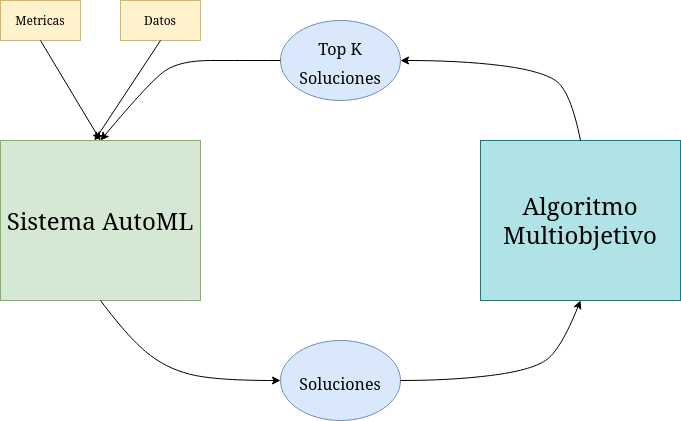
\includegraphics[scale=0.5]{Pictures/automl_moo_proposal.png}
    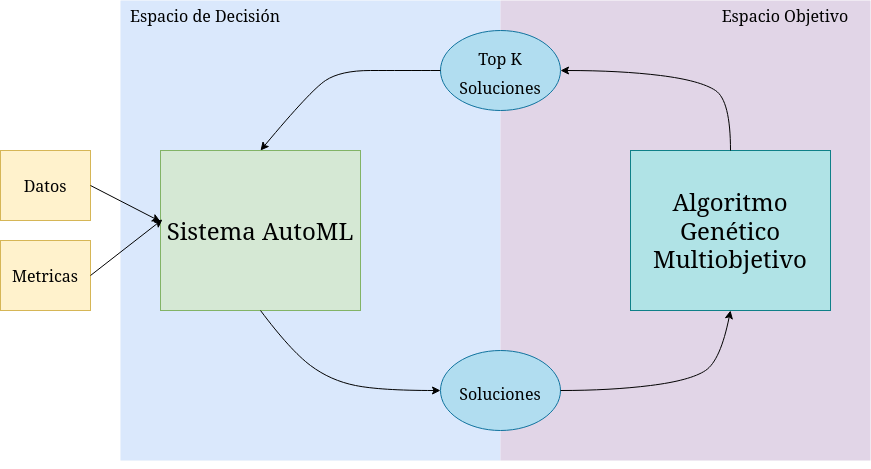
\includegraphics[scale=0.4]{Pictures/automl_moo_proposal2.png}
    \caption{Flujo general de la propuesta}
    \label{proposal:fig:flux}
\end{figure}

La soluci\'on propuesta (ver \ref{proposal:fig:flux}) est\'a compuesta por dos elementos fundamentales:
\begin{enumerate}
    \item Un sistema AutoML capaz de generar y evaluar m\'ultiples soluciones basado en un corpus de datos y un conjunto de m\'etricas. Generar nuevas soluciones partiendo de las soluciones m\'as aptas de la generaci\'on anterior.
    \item Un algoritmo de ordenaci\'on multiobjetivo capaz de funcionar solamente con el espacio objetivo y obtenga soluciones igualmente distribuidas a lo largo del frente de Pareto.
\end{enumerate}

La propuesta en cada iteraci\'on utiliza la evaluaci\'on de las soluciones generadas por el sistema de AutoML. La evaluaci\'on de una soluci\'on se representa como un vector $v$ de $m$ componentes donde $v_i$ es la evaluaci\'on de la soluci\'on con respecto a la m\'etrica $i$. El algoritmo ordena estos vectores utilizando alg\'un MOEA y retorna una lista ordenada de estos. Este proceso se repite hasta que se cumpla alg\'un criterio de parada.

La separaci\'on  por espacios existente entre ambas componentes de la propuesta permite que sean intercambiables. Todo sistema de AutoML que cumpla con estas condiciones es apto para la propuesta, no importa si est\'a enfocado en resolver el problema NAS o el problema CASH y toda algoritmo multiobjetvo capaz de producir ordenaciones efectivas utilizando solamente el espacio objetivo puede ser utilizado.
%generalizar el problema a cualquier tipo de sistema AutoML o funci\'on de ordenaci\'on.

% En su primera iteraci\'on el sistema AutoML debe producir una serie de soluciones y sus evaluaciones respectivas frente a las criterios de entrada. El algoritmo multiobjetivo debe ser capaz de ordenar efectivamente las soluciones de acuerdo a su evaluaci\'on tal que que los primeros $k$ elementos sean los m\'as aptos de para resolver el problema. Estas soluciones de mejor rendimiento se utilizan como entrada al sistema AutoML para que produzca una nueva generaci\'on de soluciones tomando la soluciones de entrada como referencia. El proceso se repite hasta que se cumpla el criterio de parada en donde se retornan los mejores individuos encontrados hasta el momento.

\subsection{Descripci\'on Formal}
El sistema propuesto est\'a compuesto por un sistema de Aprendizaje de M\'aquina Automatizado $\mathcal{A}(D, M, P)$  y un algoritmo evolutivo multiobjetivo $\mathcal{H}(TP)$. Los par\'ametros de entrada $D = \{(x_1, y_1), ..., (x_n, y_n)\}$ representa el conjunto de datos de entrada, $M = \{f_1, f_2, ..., f_m\}$ un conjunto de m\'etricas a evaluar, $P = \{p_1, p_2, ..., p_k\}$ el conjunto de soluciones de mejor rendimiento producidas por  $\mathcal{A}$ en la iteraci\'on anterior. $\mathcal{H}$ toma como entrada $TP$ que representa el conjunto de soluciones producidas en la iteraci\'on actual tras aplicar $\mathcal{A}(D, M, P)$. 
 %El objetivo final del sistema es producir una conjunto de soluciones de Aprendizaje Autom\'atico $P'$ que sean una muestra representativa del frente de Pareto (\ref{background:def:pareto_front}) utilizando un algoritmo multiobjetivo  $\mathcal{H}$ tal que $\mathcal{H}(TP) = P'$ en cierto n\'umero de iteraciones determinado por un criterio de parada. 
\begin{algorithm}[ht]\caption{Soluci\'on a AutoML Heter\'ogeneo Multiobjetivo}
    \KwIn{$\mathcal{A}$, D, M}
    \KwOut{P}
    $TP \gets \mathcal{A}(D, M, \emptyset)$ \tcp*{Se obtiene poblaci\'on inicial aleatoria}
    \While{no se cumplan condiciones de parada}{
        $P = \mathcal{H}(TP)$ \tcp*{Se extraen los m\'as aptos de una poblaci\'on} 
        $TP = \mathcal{A}(D, M, P)$ \tcp*{Se genera una nueva poblaci\'on}
    }
\end{algorithm}

% Tambi\'en debe ser capaz de entender las carectr\'isticas que componen las soluciones m\'as aptas tal que en las subsecuentes iteraciones estas se conserven. Lograr esto \'ultimo requiere que el sistema tenga en cierta medida una implementaci\'on de algoritmos gen\'eticos para construir sus soluciones, por ende, la propuesta se adapta mejor a sistemas AutoML que utilizen programaci\'on evolutiva.

\section{MOEA}
%El algoritmo trabaja con vectores debido a que optimiza para varias m\'etricas, y no con un escalar que es trivial organizar. Como se meciona en \ref{background:def:moo} se hablar ahora de dominaci\'on y el adecuado ordenamiento es vital para escoger puntos del espacio que: (i) pertenzcan a los mejores frentes, (ii) que sean los elementos representativos del frente

Esencialmente cualquier tipo de MOEA que sea suficiente informaci\'on sobre espacio objetivo se puede utilizar. Especif\'icamente para esta propuesta utilizamos una adaptaci\'on de NSGA-II (\cite{deb2002fast}) por ser un algoritmo que sigue una idea intuitiva y tiene un buen rendimiento general, suficiente para demostrar la efectividad de la propuesta.

\subsection{NSGA-II}
NSGA-II (\cite{deb2002fast}) es un algoritmo multiobjetvo basados en el frente de Pareto caracter\'isticos por dividir el proceso de selecci\'on de los individuos m\'as aptos en dos etapas:
\begin{itemize}
    \item \textit{Non Dominated Sorting} donde divide a la poblaci\'on basado en sus diferentes niveles de dominaci\'on.
    \item \textit{Crowding Distance Sorting} donde se dedicada a preservar la diversidad entre los individuos encontrados. 
\end{itemize}


\subsubsection{Non Dominated Sorting}
Durante esta etapa se agrupan las soluciones de acuerdo a su \'indice o nivel de dominaci\'on. Dicho \'indice est\'a  determinado por la cantidad de soluciones diferentes que la dominan.

\begin{definition}
    \label{proposal:def:domination_index}
    Dado un vector $x$ y un conjunto $Y$ de vectores en el espacio objetivo $\mathcal{Y}$ tal que los vectores en $Y$ dominan a $x$ (i.e. $Y = \{y | y \succ x\}$) se dice que $Ind(x) = |Y|$.
\end{definition}

\begin{definition}
    \label{proposal:def:rank_front}
    El conjunto de todas la soluciones con un mismo \'indice de dominaci\'on $i$ se les dice frente de rango $i$:
    \begin{equation*}
         F^i = \{x | x \in \mathcal{Y}, Ind(x) = i\}
    \end{equation*}
\end{definition}

El primer paso de \textit{Non Dominated Sorting} es calcular el \'indice de dominaci\'on de todas las soluciones revisando todos los pares de vectores $x, y \in \mathcal{Y}$ a la vez que se crea un grafo dirigido entre estos tal que existe una arista entre las soluciones $x$ y $y$ si $x \prec y$. Luego partiendo de las soluciones con nivel de dominaci\'on 0, visita todas las soluciones que estas dominan y les reduce el \'indice en uno. El proceso se repite hasta que no queden soluciones por analizar.
El resultado de esta primera etapa es una lista ordenada  $F = \{F^0, ..., F^k\}$ de todos los frentes de distinto rango obtenidos. 

%$F^0$ contiene las mejores vectores a los cuales nadie domina e idealmente ser\'ia una aproximaci\'on al frente de Pareto.

%Es importante entender para la correctitud del aloritmo anterior  que las soluciones que conforman un frente de rango $i$ no se \textit{Pareto dominan} ($\prec$) entre si.
%Es f\'acilmente demostrable que la \texit{Pareto dominacion (i.e. $\prec$)} cumple con la propiedad de transitividad (i.e. si $x \prec y$, $y \prec z$, entonces $x \prec z$) 
%\begin{theorem}
%Dado $P^i$, frente de rango $i$, resultado de efectuar obtenido por Non Dominated Sort sobre una conjunto soluci\'on entonces $\neg \exists x, y \in P^i$ tal que $x \prec y$
%\end{theorem}
%% Definir correctamente la prueba
%Dado un frente de rango $i$ $F_i$, tal que existen soluciones $x, y \in F_i$ se asume que $x \prec y$. Como el \'inidice de dominaci\'on de $x$ es $i$ y $x \prec y$ y ($\prec$) es una operador transitivo entonces todos los que dominan a $x$ dominan a $y$, adem\'as del propio $x$, por tanto el inidice de dominaci\'on de $y$ ser\'ia $i+1$ lo que es una contradicci\'on porque $y \in F_i$. 

\subsubsection{Crowding Distance Sorting}
\textit{Crowding Distance Sorting}(CD), uno de los aportes claves hechos por NSGA-II, se utiliza sobre  $F^i$ un frente de rango $i$ obtenido en la etapa anterior con el objetivo de ordenar sus elementos seg\'un cuan representativos del conjunto sean. Esta parte es vital pues permite que en los casos donde haya que utilizar solo la porci\'on de un frente, se utilize la m\'as representativa de este manteniendo la diversidad del conjunto.
%En la segunda etapa los vectores de cada frente obtenido se organizan utilizando \textit{crowding distance} (CD), uno de las contribuciones claves de NSGA-II (\cite{deb2002fast}). El prop\'osito de \textit{crowding distance} es estimar la densidad de las soluciones con respecto sus soluciones vecinas de tal manera que los primeros lugares pertenezcan a los elementos m\'as representativos de dicho frente.

% Imagen de crowding distance
Calcular el CD de cada soluci\'on require ordenarlas seg\'un su valor normalizado por cada funci\'on objetivo y calcular el promedio de la distancia entre una soluci\'on y sus dos adyacentes respecto a dicha funci\'on objetivo. Esta distancia es el per\'imetro del cuboide formado utilizando los vecinos m\'as cercanos como v\'ertices. Los puntos que representan el m\'inimo y m\'aximo de al menos alguna funci\'on objetivo se les asigna \textit{crowiding distance} infinita. El  algoritmo queda descrito en \ref{proposal:alg:cd}.

\begin{algorithm*}[ht]
    \caption{Crowding Distance Sorting}
    \label{proposal:alg:cd}

    \tcp{F como entrada representa un frente de rango i}
    \KwIn{F} 
    \tcp{SF como salida representa el frente ordenado seg\'un CD}
    \KwOut{SF}
    \For{i desde 0 hasta $|F|$}{
        $F[i].dist \gets 0$ \;
    } 

    \ForEach{funcion objetivo $m$}{
        $F \gets ordenar(F, m)$ \tcp*{se ordena F con respecto a m}
        $F[0].dist \gets \infty$\;
        $F[|F|].dist \gets \infty$\;

        \For{i desde 2 hasta $|F| - 1$} {
            \begin{math}
                F[i].distance  = F[i].distance + \frac{(F[i + 1].m - F[i - 1].m)}{f^{max}_{m} - f^{min}_m}
            \end{math}
        }
    }
    $SF \gets ordenar(F, dist)$ \tcp*{se ordena F respecto a CD}
\end{algorithm*}

\subsubsection{Ciclo Prinicipal}
Inicialmente se crea una poblaci\'on aleatoria $P_0$ de soluciones de tama\~no $N$. Cada soluci\'on es ordenada de acuerdo a \textit{Non Dominated Sorting} y se aplica un torneo binario utilizando operadores gen\'eticos de selecci\'on, recombinaci\'on y mutaci\'on para crear una poblaci\'on decendiente $Q_0$ de tama\~no $N$.

Luego se forma una poblaci\'on $R_t = P_t \cup Q_t$ de tama\~no 2N. La poblaci\'on $R_t$ es ordenada de acuerdo al nivel de dominaci\'on de cada individuo obteni\'endose una lista de frentes de distinto rango $F = \{F^0, ..., F^k\}$. Las soluciones en $F^0$ representan las mejores soluciones encontradas por el algoritmo hasta el momento y es necesario que pasen a formar parte de la poblaci\'on de la siguiente iteraci\'on $P_{t+1}$. Si $|F^0| < N$ el frente completo pasa formar parte de $P_{t+1}$. Los miembros restantes de la nueva poblacion son escogidos de los dem\'as frentes acorde a su \'indice de dominaci\'on. Si $F^k$ no capaz de pertencer completo a $P_{t+1}$ debido a que $\sum_0^k |F^i| > N$ se aplica \textit{Crowding Distance Sorting} sobre $F^k$ y se llena las posiciones restantes con los individuos de mayor distancia.

La nueva poblaci\'on $P_{t+1}$ se utiliza para producir una poblci\'on $Q_{t+1}$ con operadores de selecci\'on, cruzamiento y mutaci\'on. El procedimiento general de NSGA-II se muestra en la figura \ref{proposal:fig:nsga2}.

\begin{figure}[ht]
    \centering
    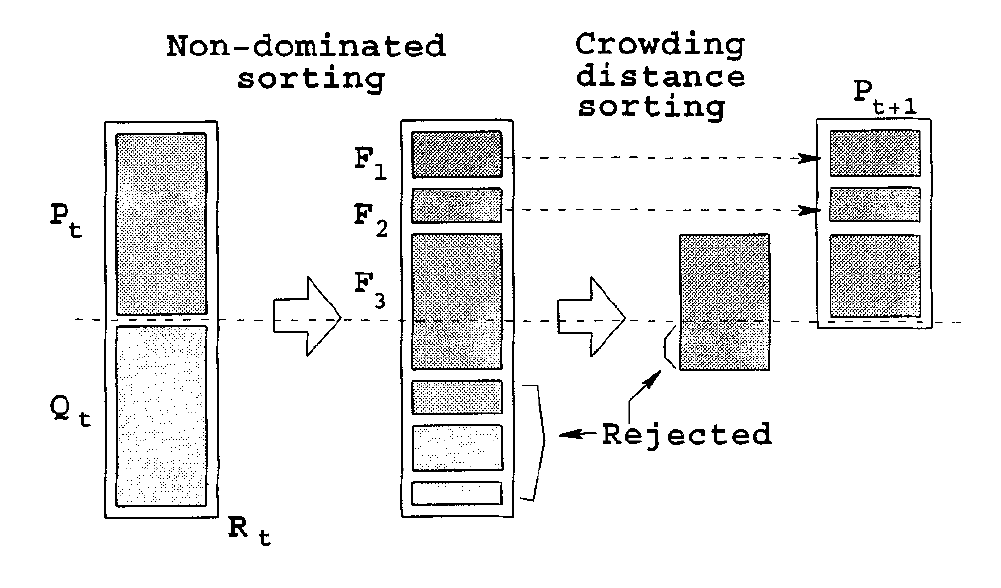
\includegraphics[scale=0.5]{Pictures/nsga2.png}
    \caption{Funcionamineto de NSGA-II}
    \label{proposal:fig:nsga2}
\end{figure}

\subsection{NSGA-II Generalizado}

NSGA-II realiza una serie de asunciones sobre las poblaciones con las que trabajan que no lo hacen perfectamente integrable con nuestra propuesta. Proponemos una adaptaci\'on del algoritmo que conserva sus dos etapas de ranking fundamentales pero con un ciclo principal m\'as sencillo que no aplica operadores gen\'eticos ni modificaciones sobre la poblaci\'on limit\'andolo al espacio objetivo $\mathcal{Y}$.

\subsubsection{Ciclo Prinicipal}
El ciclo de nuestra propuesta recibe una poblaci\'on inicial $P$ de tama\~no N y pasa directamente a aplicar \textit{Non Dominated Sorting} con los que se obtiene una lista de frentes de distinto rango $F = \{F^0, ..., F^l\}$ con el objetivo de formar un conjunto $P'$ de tama\~no $k$ que representen los mejores elementos de $P$. Las soluciones que pasan a formar parte de $P'$ se escojen a\~nadiendo en grupos por cada frente $F^i$ hasta que cierto frente $F^q$ que no pueda a\~nadirse completo. Los puestos restantes se llenan con los elementos de mayor distanica de $F^q$ tras aplicar \textit{Crowding Distance}.

Se simplifica el ciclo respetando la idea de la propuesta general.  Los sistemas AutoML son los que deciden como generar soluciones y que hacer con la informaci\'on de los m\'as aptos, permitiendo que se puedan utilizar como una caja negra intercambiable.
